\documentclass[crop,tikz]{standalone}
\begin{document}
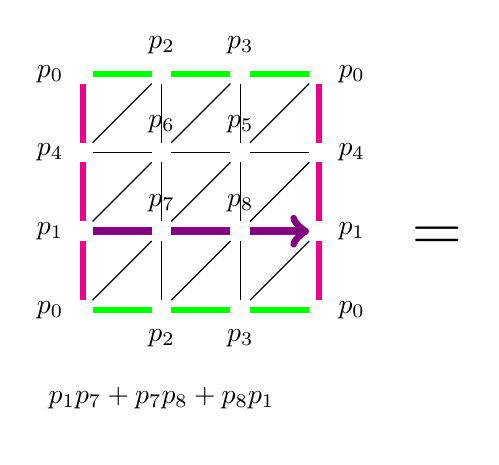
\begin{tikzpicture}
  \node (p0) at (0,0) [label=left:$p_0$]{};
  \node (p1) at (0,1) [label=left:$p_1$]{};
  \node (p2) at (1,0) [label=below:$p_2$]{};
  \node (p3) at (2,0) [label=below:$p_3$]{};
  \node (p4) at (0,2) [label=left:$p_4$]{};

  \node (p7) at (1,1) [label=above:$p_7$]{};
  \node (p8) at (2,1) [label=$p_8$]{};
  \node (p5) at (2,2) [label=$p_5$]{};
  \node (p6) at (1,2) [label=$p_6$]{};

  \node (p0p) at (3,0) [label=right:$p_0$]{};
  \node (p0ppp) at (3,3) [label=right:$p_0$]{};
  \node (p0pp) at (0,3) [label=left:$p_0$]{};
  \node (p1p) at (3,1) [label=right:$p_1$]{};
  \node (p2p) at (1,3) [label=above:$p_2$]{};
  \node (p3p) at (2,3) [label=above:$p_3$]{};
  \node (p4p) at (3,2) [label=right:$p_4$]{};

   \draw[magenta, line width = 2] (p0) -- (p1);
   \draw[magenta, line width = 2] (p0p) -- (p1p);
   \draw[magenta, line width = 2] (p1) -- (p4);
   \draw[magenta, line width = 2] (p1p) -- (p4p);
   \draw[magenta, line width = 2] (p4) -- (p0pp);
   \draw[magenta, line width = 2] (p4p) -- (p0ppp);

   \draw[green, line width = 2] (p0) -- (p2);
   \draw[green, line width = 2] (p2) -- (p3);
   \draw[green, line width = 2] (p3) -- (p0p);
   \draw[green, line width = 2] (p0pp) -- (p2p);
   \draw[green, line width = 2] (p2p) -- (p3p);
   \draw[green, line width = 2] (p3p) -- (p0ppp);

   \draw (p1) -- (p7);
   \draw (p0) -- (p7);
   \draw (p2) -- (p7);

   \draw (p2) -- (p8);
   \draw (p7) -- (p8);
   \draw (p3) -- (p8);

   \draw (p3) -- (p1p);
   \draw (p8) -- (p1p);
   \draw (p8) -- (p4p);
   \draw (p8) -- (p5);

   \draw (p1) -- (p6);
   \draw (p4) -- (p6);
   \draw (p7) -- (p6);

   \draw (p6) -- (p5);
   \draw (p7) -- (p5);
   \draw (p8) -- (p5);

   \draw (p5) -- (p4p);
   \draw (p5) -- (p0ppp);
   \draw (p5) -- (p3p);

   \draw (p6) -- (p3p);
   \draw (p6) -- (p2p);
   \draw (p4) -- (p2p);

   \draw[violet, line width=3, ->] (p1) -- (p7) -- (p8)  -- (p1p);

   \node (text) at (4.5,.5) [label={\fontsize{30}{40}\selectfont$=$}]{};
   \draw (text);

   \node (name) at (1,-1.5) [label=$p_1 p_7 + p_7 p_8 + p_8 p_1$]{};
   \draw (text);
\end{tikzpicture}
\end{document}
